%instiki:category: FisicaSubatomica
\chapter{Ruptura espont\'anea de simetr\'\i a}
\label{rupt-espont-de} %noinstiki
%instiki:
%instiki:***
%instiki:
%instiki:[[NotasFS|Tabla de Contenidos]]
%instiki:
%instiki:***
%instiki:
%instiki:* [Masa para el campo escalar](#masa-para-el)
%instiki:
%instiki:* [Bos\'on de Goldstone](#boson-de-goldstone)
%instiki:
%instiki:* [Masa para el bos\'on gauge](#masa-para-el-1)
%instiki:
%instiki:* [Mecanismo de Higgs en un caso no Abeliano](#mecanismo-de-higgs)
%instiki:
%instiki:***
%instiki:



\section{Campo escalar real}
\begin{frame}[fragile,allowframebreaks]
Escribamos el Lagrangiano para una partícula escalar real de masa $m$ como
\begin{equation}
\label{eq:83qft}
\mathcal{L}=\tfrac{1}{2}\partial^\mu\phi\partial_\mu\phi-V(\phi)
\end{equation}
con
\begin{equation}
  V(\phi)=\tfrac{1}{2}\mu^2\phi^2.
\end{equation}
Este Lagrangiano es simétrico bajo la transformación discreta $\phi\to-\phi$. 

Cuando $\mu^2\gt 0$, el campo tiene excitaciones alrededor del mínimo del potencial que cuestan energía y dicho término se interpreta como la masa de la partícula. Ver figura \ref{fig:x2}. En Teoría Cuántica de Campos al estado de mínima energía se le llama el vacío y las excitaciones alrededor del vació corresponden a las partículas.
%noinstiki
\begin{figure} %noinstiki
  \centering %noinstiki
  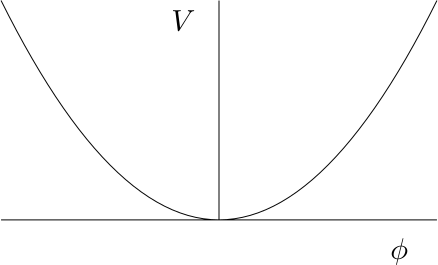
\includegraphics[scale=0.8]{vphi2}
  \caption{$V(\phi)=\frac{1}{2}\mu^2 \phi^2$ con $\mu^2\gt 0$} %noinstiki
  \label{fig:x2} %noinstiki
\end{figure} %noinstiki <div id="fig:x2">Figura: Un mínimo</div>
%noinstiki![cuerda](http://gfif.udea.edu.co/figfs/vphi2.png)
%noinstiki

Si $\mu^2\lt 0$, no existe un mínimo del potencial alrededor del cual el campo pueda oscilar. Además el alejamiento del campo del punto de simetría del potencial no cuesta energía. Por consiguiente en ese caso, el término de interacción
\begin{equation}
  V(\phi)=\tfrac{1}{2}\mu^2   \qquad 
  \mu^2\lt 0,
\end{equation}
no puede interpretarse como un término de masa en el Lagrangiano dado por la ec.~\eqref{eq:83qft}. 

Consideremos ahora el potencial
\begin{equation}
  V(\phi)=\tfrac{1}{2}\mu^2\phi^2+\tfrac{1}{4}\lambda\phi^4
  \qquad   \mu^2\lt 0,\ \lambda\gt 0
\end{equation}
que mantiene la simetría bajo la transformación discreta $\phi\to-\phi$. $\lambda\gt 0$ garantiza la aparición de los dos mínimos que se muestran el la figura \ref{fig:x2l}. Si la energía es suficientemente alta como se muestra en la figura~\ref{fig:x2l}, las excitaciones son simétricas con respecto al máximo del potencial y el término en $\mu^2$ no puede interpretarse como masa para la partícula escalar. 

%noinstiki
\begin{figure} %noinstiki
  \centering %noinstiki
  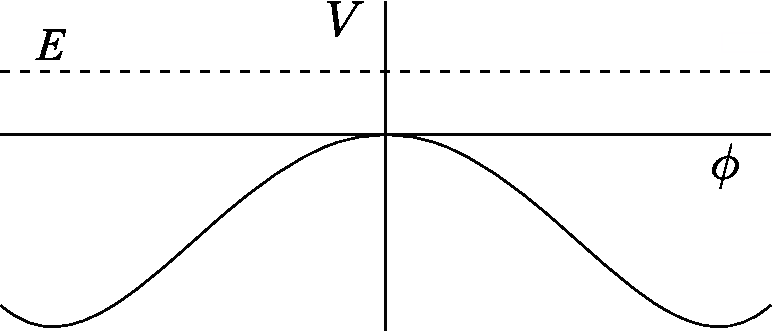
\includegraphics{vphi4}
  \caption{$V(\phi)=\frac{1}{2}\mu^2 \phi^2+\frac{1}{4}\lambda\phi^4$ con $\mu^2\lt 0$, y $\lambda\gt 0$. Simetría exácta} %noinstiki
  \label{fig:x2l} %noinstiki
\end{figure} %noinstiki <div id="fig:x2l">Figura: Mínimos degenerados</div>
%noinstiki![cuerda](http://gfif.udea.edu.co/figfs/vphi4.png)
%noinstiki
Sin embargo, si la energía es suficientemente baja como se muestra en la figura~\ref{fig:x2lm}, las excitaciones alrededor del mínimo dan lugar a la aparición de un término de masa para el campo escalar. Además, dichas excitaciones no respetan la simetrías $\phi\to-\phi$. En tal caso decimos que la simetría ha sido espontáneamente rota: aunque el Lagrangiano mantiene la simetría original, el vacío la rompe. 

%noinstiki
\begin{figure} %noinstiki
  \centering %noinstiki
  %noinstiki
  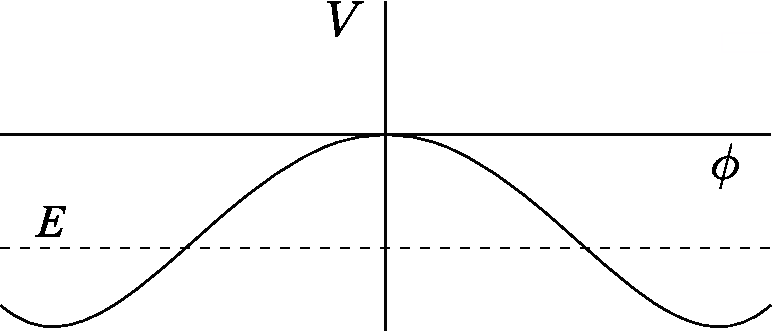
\includegraphics{vphi4m}
  \caption{$V(\phi)=\frac{1}{2}\mu^2 \phi^2+\frac{1}{4}\lambda\phi^4$ con $\mu^2\lt 0$, y $\lambda\gt 0$. Simetría espontáneamente rota.} %noinstiki
  \label{fig:x2lm} %noinstiki
\end{figure}  %noinstiki <div id="fig:x2lm">Figura: Simetría espontáneamente rota  </div>
%noinstiki![vphi4lm](http://gfif.udea.edu.co/figfs/vphi4lm.png)
%noinstiki

Para analizar cuantitativamente el espectro de partículas es necesario expandir el campo alrededor del mínimo y determinar las excitaciones. Establezcamos en primer lugar los mínimos del potencial. La $\partial V/\partial\phi=0$ da lugar a
\begin{align}
  \mu^2\phi+\lambda\phi^3&=0\\
  \phi(\mu^2+\lambda\phi^2)&=0,
\end{align}
con extremos $\phi_{\text{max}}=0$, y 
\begin{equation}
  \label{eq:90qft}
  \phi_{\text{min}}\equiv\langle\phi\rangle\equiv v=\pm\sqrt{\frac{-\mu^2}{\lambda}}.
\end{equation}
De hecho 
\begin{equation}
  \frac{\partial^2V}{\partial\phi^2}=\mu^2+3\lambda\phi^2.
\end{equation}
$\phi=0$ corresponde a un máximo, mientras que la segunda derivada para $\phi=\pm\sqrt{-\mu^2/\lambda}$ es $-2\mu^2\gt 0$ y corresponden a los mínimos. Expandiendo el campo alrededor del mínimo
\begin{equation}
  \phi(x)=H(x)+v
\end{equation}
\begin{align}
  V(\phi)=&\tfrac{1}{2}\mu^2 \phi^2+\tfrac{1}{4}\lambda\phi^4\nonumber\\
  =&\tfrac{1}{2}\mu^2 (H+v)^2+\tfrac{1}{4}\lambda(H+v)^4\nonumber\\
  =&\tfrac{1}{2}\mu^2 (H+v)^2+\tfrac{1}{4}\lambda(H+v)^4\nonumber\\
  =&\tfrac{1}{2}\mu^2 \left(H^2+2vH+v^2\right)+\tfrac{1}{4}\lambda\left(H^2+2vH+v^2\right)^2\nonumber\\
  =&\tfrac{1}{2}\mu^2 \left(H^2+2vH+v^2\right)+\tfrac{1}{4}\lambda\left[H^4+2H^2\left(2vH+v^2\right)+\left(2vH+v^2\right)^2\right]\nonumber\\
  =&\tfrac{1}{2}\mu^2 \left(H^2+2vH+v^2\right)+\tfrac{1}{4}\lambda\left[H^4+4vH^3+2H^2v^2+4v^2H^2+4v^3H+v^4\right]\nonumber\\
  =&\tfrac{1}{2}\mu^2 \left(H^2+2vH+v^2\right)+\tfrac{1}{4}\lambda\left[H^4+4vH^3+6H^2v^2+4v^3H+v^4\right]\nonumber\\
  =&\tfrac{1}{2}\mu^2H^2-\tfrac{3}{2}H^2\mu^2+\mu^2vH-\mu^2vH+\tfrac{1}{2}\mu^2v^2-\tfrac{1}{4}\mu^2v^2+\tfrac{1}{4}\lambda\left[H^4+4vH^3\right]\nonumber\\
\label{eq:84qft}
V(H)=&\tfrac{1}{2}\left(-2\mu^2\right)H^2+\lambda vH^3+\tfrac{1}{4}\lambda H^4+\tfrac{1}{4}\mu^2v^2,
\end{align}
y
\begin{equation}
  \label{eq:88qft}
  \mathcal{L}_H=\tfrac{1}{2}\partial^\mu H\partial_\mu H-\tfrac{1}{2}\left(-2\mu^2\right)H^2-\lambda vH^3-\tfrac{1}{4}\lambda H^4+\text{constant}.
\end{equation}
Entonces $H$ adquiere una masa $-2\mu^2$ y no es invariante bajo $H\to-H$. 

Otro método es usar las ecuaciones de mínimo $-\mu^2=\lambda v^2$, para eliminar un parámetro del potencial:
\begin{align}
  V(\phi)&=-\tfrac{1}{2}\lambda v^2\phi^2+\tfrac{1}{4}\lambda\phi^4\nonumber\\
  =&-\tfrac{1}{2}\lambda v^2 \left(H^2+2vH+v^2\right)+\tfrac{1}{4}\lambda\left[H^4+4vH^3+6H^2v^2+4v^3H+v^4\right]\nonumber\\
  =&\lambda v^2H^2+\lambda vH^3+\tfrac{1}{4}\lambda H^4+\text{constant}.
\end{align}
Podemos escribir el potencial en términos del  nuevo campo como
\begin{align}
\label{eq:higgspot}
  V(H)=\frac{1}{2}m_H^2H^2+\frac{1}{2}\frac{m_H^2}{v}H^3+\frac{1}{8}\frac{m_H^2}{v^2} H^4\,.
\end{align}
donde
\begin{equation}
\label{eq:higgsmass}
  m_H^2=2\left|\mu^2\right|=2\lambda v^2
\end{equation}

\subsection{Ausencia de taquiones}

Uno se podría preocupar por la presencia de un término de masa
imaginaria en el Lagrangiano, pero como estamos hablando de
transiciones de fase, estos porcesos deben suceder en presencia de
temperatura, por ejemplo la temperatura asociada al universo primitivo
durante las fases tempranas del Big Bang. En presencia de temperatura,
todas las partículas adquieren una masa térmica proporcional a la
temperatura como resultado de su interacción con el plasma. De este
modo, a altas temperaturas la masa de la partícula escalar esta
dominada por la temperatura y al ser positiva el potencial escalar
tiene un único mínimo simétrico. Cuando la temperatura baja lo
suficiente para que la masa al cuadrado negativa domine, el mínimo se
convierte en un máximo local altamente inestable y ocurre muy
rapidamente la transición de fase al nuevo mínimo no simétrico donde
la masa del escalar esta bien definida.

\subsection{Caso complejo}


Consideremos ahora un campo escalar complejo sin término de masa, pero con potencial:
\begin{equation}
  \label{eq:85qft}
  \mathcal{L}=\partial^\mu\phi^*\partial_\mu\phi-V(\phi)
\end{equation}
\begin{equation}
  V(\phi)=\mu^2\phi^*\phi+\lambda(\phi^*\phi)^2 
  \qquad 
  \mu^2\lt 0,\ \lambda\gt 0 
\end{equation}
La simetría del Lagrangiano corresponde a $U(1)$ global. Este potencial corresponde al ``sombrero mexicano'', como se ilustra en la Figura \ref{fig:mexicanhat}. Para una energía suficientemente baja de manera que el campo deba oscilar alrededor del mínimo aparecen dos tipos de excitaciones. Una sobre las paredes  que cuestan energía y corresponden a un campo escalar masivo como en el caso anterior, y otra a lo largo de la circunferencia de mínimo, que corresponde a una partícula escalar sin masa, y es llamada bosón del Golstone. 



\begin{figure}
  \centering
  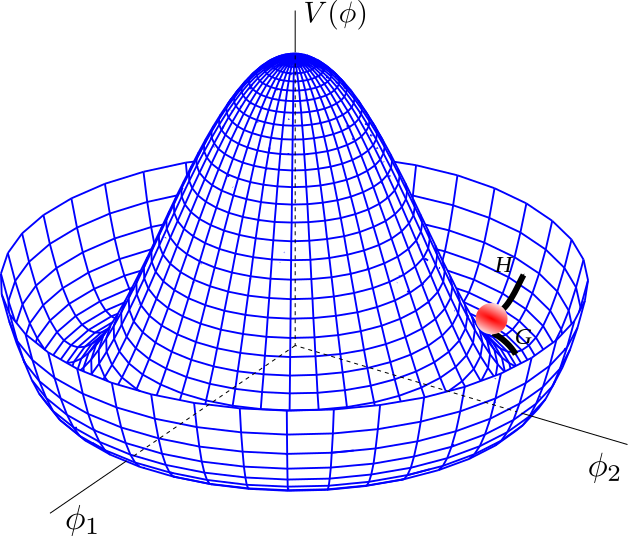
\includegraphics[scale=0.5]{mexicanhat}
  \caption{Potential for complex scalar field}
  \label{fig:mexicanhat}
\end{figure}



El Lagrangiano escalar complejo es equivalente al Lagragiano de dos campos escalares reales con los mismos paramétros. Para un conjunto de $N$ campos reales tenedremos (suma sobre $i$) \cite{Peskin}\footnote{§ 11.1}: 
\begin{align}
  \mathcal{L}=\frac{1}{2}\partial^\mu\phi^i\partial_\mu\phi_i-\frac{1}{2}\mu^2\phi_i\phi^i-\frac{1}{2}\mu^2\left(\phi_i\phi^i\right)^2\,,
\end{align}
que es invariante bajo una simetría $O(N)$
\begin{align}
  \phi^i\to{\phi'}^i=R^{ij}\phi^j\,,
\end{align}
para cualquier matriz $N\times  N$ ortogonal $R$. El análisis para $N=2$ da lugar a un bosón de Goldstone. El anális para $N>2$ es el mismo y por cada campo real que se introduzca aparece un nuevo bosón de Goldstone \cite{Peskin}:
\begin{quote}
  [\ldots] there are not continuous symmetries for $N=1$, while for $N=2$ there is a single direction of rotation. A rotation in $N$ dimensions can be in any one of $N(N-1)$ planes, so the $O(N)$--symmetric theory has $N(N-1)/2$ continuous symmetries. After spontaneous symmetry breaking there are $(N-1)(N-2)/2$  remaining symmetries corresponding to rotations of the $(N-1)$ [non massive] fields. The number of \emph{broken} symmetries is the difference, $N-1$.
\end{quote}
Entonces tenemos el siguiente teorema \cite{Peskin}
\begin{quote}
\emph{Goldstone's theorem states that for every spontaneously broken continuous symmetry, the theory must contain a massless particle.}
\end{quote}

Also from \cite{Peskin}\footnote{Introduction to Chapter 20}
\begin{quote}
  In a global symmetry  that is spontaneously broken the symmetry currents are still conserved and interactions are similarly restricted [the Lagrangian keeps the symmetry], but the vacuum state does not respect the symmetry and the particles do not form obvious symmetry multiplets. Instead, such a theory contains massless particles, Goldstone bosons, one for each generator of the spontaneously broken symmetry. The third case is that of a local, or gauge, symmetry. [\ldots] such a symmetry requires the existence of a massless vector field for each symmetry generator, and the interactions among these fields are highly restricted.

It is now only natural to consider a fourth possibility: What happens if we include both local gauge invariance  and spontaneous symmetry breaking in the same theory?
\end{quote}
 

En el caso de la Acción invariante gauge local bajo el Grupo $U(1)$, tenemos el Lagrangiano 
\begin{equation}
  \label{eq:89qft}
  \mathcal{L}=\left(\mathcal{D}^\mu\phi\right)^*\mathcal{D}_\mu\phi-\mu^2\phi^*\phi-\lambda\left(\phi^*\phi\right)^2-\tfrac{1}{4}F^{\mu\nu}F_{\mu\nu}
  \qquad 
  \mu^2\lt 0\text{ and } \lambda\gt 0\,.
\end{equation}
Este es el Lagrangiano más general posible para un campo escalar complejo y el campo $A_\mu$ que deja la Acción invariante de Lorentz e invariante bajo la transformación gauge $U(1)$
\begin{align}
\label{eq:sqedgu}
  \phi(x)\to \phi'(x)=e^{i\theta(x)} \phi(x)\,,
\end{align}
y da lugar a la electrodinámica cuántica escalar.


\subsection{Gauge unitario}
Como $\phi$ es un campo complejo, podemos escribirlo en coordenadas polares con un campo real asociado a la magnitud del campo complejo y otro a la fase
\begin{align*}
  \phi(x)=\varphi(x)e^{i\eta(x)}
\end{align*}
Expandiendo el campo $\varphi(x)$ alrededor del mínimo: $\varphi(x)=(H(x)+v)/\sqrt{2}$, tenemos
\begin{align*}
    \phi(x)=e^{i\eta(x)}\left(\frac{H(x)+v}{\sqrt{2}}\right)\,.
\end{align*}


La libertad gauge nos permite en un momento determinado escoger la fase $\theta(x)$ de la ec.~\eqref{eq:sqedgu} sin que ese alteren los observables de la teoría. Para el campo en coordenadas polares tenemos que
\begin{align*}
     \phi\to\phi'=e^{i\theta(x)}e^{i\eta(x)}\left(\frac{H(x)+v}{\sqrt{2}}\right)
\end{align*}
Haciendo $\theta(x)=-\eta(x)$,
\begin{equation}
\label{eq:87qft}
   \phi\to\phi'=e^{-i\eta(x)+i\eta(x)}\left(\frac{H(x)+v}{\sqrt{2}}\right)=\frac{H(x)+v}{\sqrt{2}}
\end{equation}
\begin{align}
  \mathcal{L}\to\mathcal{L}' &=\left[\left(\mathcal{D}^\mu\right)'\phi'\right]^*\left(\mathcal{D}_\mu\right)'\phi'-\mu^2\left(\phi^*\right)'\phi'-\lambda\left[\left(\phi^*\right)'\phi'\right]^2-\tfrac{1}{4}\left(F^{\mu\nu}F_{\mu\nu}\right)'\nonumber\\
 &=\tfrac{1}{2}\left[\partial^\mu H+ig{A'}^\mu(H+v)\right]\left[\partial_\mu H-ig{A'}_\mu(H+v)\right]-\tfrac{1}{2}\mu^2(H+v)^2-\tfrac{1}{4}\lambda(H+v)^4-\tfrac{1}{4}\left(F^{\mu\nu}F_{\mu\nu}\right)'\,.
\end{align}
En adelante omitiremos las primas, aunque debe estar claro que se esta trabajando en el gauge específico de la ec.~\eqref{eq:87qft}. Entonces
\begin{align}
  \mathcal{L}&=\tfrac{1}{2}\partial^\mu H\partial_\mu H-\tfrac{1}{2}\mu^2(H+v)^2-
  \tfrac{1}{4}\lambda(H+v)^4+\tfrac{1}{2}g^2A^\mu A_\mu(H+v)^2
  -\tfrac{1}{4}F^{\mu\nu}F_{\mu\nu}.
\end{align}
Usando la ec.~\eqref{eq:84qft}
\begin{equation}
  \label{eq:94qft}
  \mathcal{L}=\mathcal{L}_H+\mathcal{L}_{A^\mu}+\tfrac{1}{2}g^2A^\mu A_\mu H^2+g^2vA^\mu A_\mu H,
\end{equation}
donde $\mathcal{L}_H$ esta dado por la ec.~\eqref{eq:88qft} y
\begin{equation}
  \mathcal{L}_{A^\mu}=-\tfrac{1}{4}F^{\mu\nu}F_{\mu\nu}+\tfrac{1}{2}g^2v^2A^\mu A_\mu.
\end{equation}
Teniendo en cuenta la ec.~\eqref{eq:23qft} para el Lagrangiano de Proca, vemos que como consecuencia de la ruptura espontánea de simetría el campo gauge ha adquirido una masa
\begin{equation}
  m_{A^\mu}=gv.
\end{equation}

El mecanismo completo mediante el cual, a partir de un Lagrangiano invariante gauge local, los bosones gauge adquieren masa se llama \emph{mecanismo de Higgs} \cite{Higgs:1964pj}. La partícula escalar que adquiere masa se llama Higgs, mientras que el bosón de Goldstone es absorbido por campo gauge como modo longitudinal. 

El número de grados de libertad independientes en el Lagrangiano original en la ec.~\eqref{eq:89qft} es cuatro. Correspondientes a los dos grados de libertad del bosón gauge no masivo y los dos del campo escalar complejo. En el Lagrangiano final en la ec.~\eqref{eq:94qft} no aparece el bosón de Goldstone. Sin embargo esto no es un problema porque dicho Lagrangiano también tiene cuatro grados de libertad correspondientes a  los tres grados de libertad del bosón gauge masivo y al grado de libertad del bosón de Higgs. 

\end{frame}

\subsection{Superconductivity}

A review ot the use of the Proca Equations for a massive photon in superconductivity is given in~\cite{massivephoton}. A popularization review along this lines is in the book of Frank Wilczek ``The Lightness of Being'' (see Additional references).

The photon mass inside a superconductor is $10^{-11}\,$GeV (or 1/1000 of the electron mass according to~\cite{massivephoton}). Also from the article in Beamline $\lambda\sim 10\ \mu\text{m}$ y $M_\gamma=\hbar/\lambda c$ %check numbers

There are two important length scales in a superconductor. The first measures how efficientrly the condensate expels a magnetic field. In fact, the expulsion is not 

Additional references:
\begin{itemize}
\item The Lightness of Being: Mass, Ether, and the Unification of Forces,
Frank Wilczek, \url{http://www.amazon.com/The-Lightness-Being-Unification-Forces/dp/0465018955}
\item \url{http://www.scholarpedia.org/article/Englert-Brout-Higgs-Guralnik-Hagen-Kibble_mechanism_(history)}
\item Elementary Particle Physics: Volume 1: Quantum Field Theory and ..., Volume 1
 By Yorikiyo Nagashima, \url{Elementary Particle Physics: Volume 1: Quantum Field Theory and ..., Volume 1
 By Yorikiyo Nagashima}
\item From Superconductors 
to Supercolliders
by LANCE DIXON \url{http://www.slac.stanford.edu/pubs/beamline/26/1/26-1-dixon.pdf}
\item Electrodynamics of Superconductors \url{http://www.physics.buffalo.edu/phy514/w11/index.html}
\end{itemize}


\section{Apéndices}



\subsection{Coordenadas cartesianas}
Expandimos el campo alrededor del m\'\i nimo:

\begin{equation}
  \label{eq:193}
  \phi=\phi^0=\frac{\phi_1+i\phi_2}{\sqrt{2}}=\frac{1}{\sqrt{2}}(H(x)+v+iG)
\end{equation}
Entonces
\begin{align}
  \label{eq:194}
  V(\phi_1,\phi_2)=\tfrac{1}{2}\mu^2\left(\phi_1^2+\phi_2^2\right)
+\tfrac{1}{4}\lambda\left(\phi_1^2+\phi_2^2\right)^2
\end{align}
%\left(\right)
La condici\`on de m\'\i nimo es 
\begin{align}
  \frac{\partial V}{\partial\phi_1}=&0\nonumber\\
  =&\tfrac{1}{2}\mu^2\left(2\phi_1\right)
+\tfrac{1}{4}\lambda2\left(\phi_1^2+\phi_2^2\right)2\phi_1\nonumber\\
  =&\phi_1\left[\mu^2+\lambda\left(\phi_1^2+\phi_2^2\right)\right]
\end{align}
\begin{align}
  \frac{\partial V}{\partial\phi_2}=&0\nonumber\\
  =&\phi_2\left[\mu^2+\lambda\left(\phi_1^2+\phi_2^2\right)\right]
\end{align}
Los infinitos m\'\i nimos degenerados corresponden a la circunferencia
\begin{equation}
\phi_1^2+\phi_2^2=v^2=\frac{-\mu^2}{\lambda}
\end{equation}
El campo debe ser neutro pues, reemplazando \eqref{eq:193} en la ec.~\eqref{eq:194}
\begin{align}
  \mathcal{L}=&\tfrac{1}{2}\partial^\mu H\partial_\mu H+\tfrac{1}{2}\partial^\mu G\partial_\mu G-\tfrac{1}{2}\mu^2\left[(H+v)^2+G^2\right]-\tfrac{1}{4}\lambda\left[(H+v)^4+2(H+v)^2G^2+G^4\right]\nonumber\\
  \mathcal{L}=&\tfrac{1}{2}\partial^\mu H\partial_\mu H-\tfrac{1}{2}\mu^2(H+v)^2-\tfrac{1}{4}\lambda(H+v)^4+\tfrac{1}{2}\partial^\mu G\partial_\mu G-\tfrac{1}{2}\mu^2G^2-\tfrac{1}{4}\lambda\left[2(H+v)^2G^2+G^4\right].
\end{align}
Usando la ec.~(\ref{eq:84}), tenemos
\begin{align}
  \mathcal{L}=&\tfrac{1}{2}\partial^\mu H\partial_\mu H-\tfrac{1}{2}\left(-2\mu^2\right)H^2-\lambda vH^3-\tfrac{1}{4}\lambda H^4\nonumber\\
  &+\tfrac{1}{2}\partial^\mu G\partial_\mu G-\tfrac{1}{2}\mu^2G^2-\tfrac{1}{4}\lambda G^4\nonumber\\
  &-\tfrac{1}{2}\lambda\left[H^2G^2+2vHG^2+v^2G^2\right]+\text{constant}\nonumber\\
\end{align}
\begin{align}
    \mathcal{L}=&\tfrac{1}{2}\partial^\mu H\partial_\mu H-\tfrac{1}{2}\left(-2\mu^2\right)H^2-\lambda vH^3-\tfrac{1}{4}\lambda H^4\nonumber\\
  &+\tfrac{1}{2}\partial^\mu G\partial_\mu G-\tfrac{1}{4}\lambda G^4\nonumber\\
  &-\lambda vHG^2-\tfrac{1}{2}\lambda H^2G^2+\text{constant}\nonumber\\
\end{align}
Como antes, el campo $H$ tiene masa $2|\mu^2|$. El t\'ermino en $G^2$ ha desaparecido implicando que el campo $G$ tiene masa cero.
En este caso decimos que la invarianza $U(1)$ de la acci\'on ha sido espont\'aneamente rota
\begin{equation}
  U=e^{iY\theta},
\end{equation}
donde $Y$ es el generador de la transformaci\'on y $\theta$ el par\'ametro. Despu\'es de la ruptura espont\'anea de la simetr\'\i a diremos que el generador $Y$ ha sido roto. El campo que adquiere masa recibe el nombre de \emph{bos\'on de Higgs} \cite{Higgs:1964pj}, mientras que el campo sin masa es llamado \emph{bos\'on de Goldstone}. 

El \emph{Teorema de Goldstone} establece que por cada generador roto de una simetr\'\i a continua debe aparecer un bos\'on de Goldstone.

\subsection{Coordenadas polares}

Si hacemos
\begin{equation}
  \phi=e^{i\eta(x)}\frac{\rho(x)}{\sqrt{2}}
\end{equation}
\begin{align}
  \mathcal{L}&=\tfrac{1}{2}\left(\partial^\mu\rho-i\rho\partial^\mu\eta\right)\left(\partial_\mu\rho+i\rho\partial_\mu\eta\right)-\tfrac{1}{2}\mu^2\rho^2-\tfrac{1}{2}\lambda\rho^4\nonumber\\
    \mathcal{L}&=\tfrac{1}{2}\partial^\mu\rho\partial_\mu\rho+\tfrac{1}{2}\rho^2\partial^\mu\eta\partial_\mu\eta-\tfrac{1}{2}\mu^2\rho^2-\tfrac{1}{2}\lambda\rho^4
\end{align}


Haciendo $\rho\to \rho+v$, tenemos
\begin{align}
  \mathcal{L}=&\tfrac{1}{2}\partial^\mu\rho\partial_\mu\rho-\tfrac{1}{2}\mu^2(\rho+v)^2-\tfrac{1}{2}\lambda(\rho+v)^4\nonumber\\
  +&\tfrac{1}{2}v^2\partial^\mu\eta\partial_\mu\eta+\tfrac{1}{2}\rho^2\partial^\mu\eta\partial_\mu\eta+2v\rho\partial^\mu\eta\partial_\mu\eta\nonumber\\
  \mathcal{L}=&\tfrac{1}{2}\partial^\mu\rho\partial_\mu\rho-\tfrac{1}{2}\left(-2\mu^2\right)\rho^2-\lambda v\rho^3-\tfrac{1}{4}\lambda \rho^4\nonumber\\
  +&\tfrac{1}{2}v^2\partial^\mu\eta\partial_\mu\eta+\tfrac{1}{2}\rho^2\partial^\mu\eta\partial_\mu\eta+2v\rho\partial^\mu\eta\partial_\mu\eta
\end{align}
De nuevo no hay t\'ermino de masa para $\eta$.


%\left(\right)
%%% Local Variables: 
%%% mode: latex
%%% TeX-master: "fullnotes"
%%% End: 
